\documentclass[12pt, twoside]{article}
%\documentclass[12pt, twoside]{article}
\usepackage[letterpaper, margin=1in, headsep=0.2in]{geometry}
\setlength{\headheight}{0.6in}
%\usepackage[english]{babel}
\usepackage[utf8]{inputenc}
\usepackage{microtype}
\usepackage{amsmath}
\usepackage{amssymb}
%\usepackage{amsfonts}
\usepackage[nomessages]{fp} %\FPeval{\var-name}{2*sin(pi/6)}
\usepackage{siunitx} %units in math. eg 20\milli\meter
\usepackage{yhmath} % for arcs, overparenth command
\usepackage{tikz} %graphics
\usetikzlibrary{quotes, angles, arrows, arrows.meta}
\usepackage{pgfplots}
\usepgfplotslibrary{fillbetween}
\pgfplotsset{compat=1.16}
\usepackage{graphicx} %consider setting \graphicspath{{images/}}
\usepackage{parskip} %no paragraph indent
\usepackage{enumitem}
\usepackage{multicol}
\usepackage{venndiagram}

\usepackage{fancyhdr}
\pagestyle{fancy}
\fancyhf{}
\renewcommand{\headrulewidth}{0pt} % disable the underline of the header
\raggedbottom
\hfuzz=2mm %suppresses overfull box warnings

\usepackage{hyperref}

\fancyhead[LO]{La Scuola d'Italia / Dr.\ Huson / IB Math 12 \\* 20 October 2026}
\fancyhead[RO]{\fbox{\begin{minipage}{6cm}\footnotesize Nickname:\\[0.5cm]\end{minipage}}}
\fancyfoot[C]{\thepage}

\begin{document}
\subsubsection*{2.2 Classwork: The Cosine Rule}

\begin{center}
\fbox{\begin{minipage}{0.9\textwidth}
\centering
In triangle $ABC$, side $a$ is opposite angle $A$, side $b$ is opposite
angle $B$, and so on.
$$c^{2} = a^{2} + b^{2} - 2ab\cos C
\qquad\qquad
\cos C = \frac{a^{2} + b^{2} - c^{2}}{2ab}$$
\end{minipage}}
\end{center}

Give answers correct to three significant figures, unless they are exact.

\begin{enumerate}[itemsep=0.15cm]

%--- Problem 1: Cosine rule on three triangles: side from SAS, largest angle from SSS (obtuse), classify, exact side with 120 deg [7 marks] ---
%--- Source: Original (freshly authored, AA SL 3.2); Haese AA SL Ch. 9 ---
\item[1.]
The diagrams are not to scale.

\begin{center}
\begin{tikzpicture}[scale=0.33]
  \coordinate (A) at (0,0);
  \coordinate (B) at (11,0);
  \coordinate (C) at (6.128,5.142);
  \draw[thick] (A) -- (B) -- (C) -- cycle;
  \draw pic["$40^\circ$", draw, angle radius=0.6cm, angle eccentricity=1.75] {angle = B--A--C};
  \node[below] at (5.5,0) {$11$};
  \node[above left] at (3.064,2.571) {$8$};
  \node[above right] at (8.564,2.571) {$x$};
  \node[below] at (5.5,-1.6) {(a)};
\end{tikzpicture}
\hfill
\begin{tikzpicture}[scale=0.33]
  \coordinate (P) at (0,0);
  \coordinate (Q) at (9,0);
  \coordinate (R) at (3.167,3.869);
  \draw[thick] (P) -- (Q) -- (R) -- cycle;
  \draw pic["$\theta$", draw, angle radius=0.35cm, angle eccentricity=1.9] {angle = P--R--Q};
  \node[below] at (4.5,0) {$9$};
  \node[above left] at (1.583,1.935) {$5$};
  \node[above right] at (6.083,1.935) {$7$};
  \node[below] at (4.5,-1.6) {(b), (c)};
\end{tikzpicture}
\hfill
\begin{tikzpicture}[scale=0.33]
  \coordinate (K) at (0,0);
  \coordinate (L) at (10,0);
  \coordinate (M) at (-3,5.196);
  \draw[thick] (K) -- (L) -- (M) -- cycle;
  \draw pic["$120^\circ$", draw, angle radius=0.45cm, angle eccentricity=1.8] {angle = L--K--M};
  \node[below] at (5,0) {$10$};
  \node[left] at (-1.5,2.598) {$6$};
  \node[above right] at (3.5,2.598) {$y$};
  \node[below] at (3.5,-1.6) {(d)};
\end{tikzpicture}
\end{center}

\begin{enumerate}[itemsep=0.1cm]
  \item Find the value of $x$.
  \item Find the size of the largest angle, $\theta$, in the second triangle.
  \item State whether the second triangle is acute, right-angled or obtuse.
  \item Find the exact value of $y$.
\end{enumerate}

\begin{tikzpicture}
  \draw (-0.6,0) rectangle (14.6,9.4);
  \foreach \y in {1,2,...,9} \draw[dotted] (0,\y)--(14.1,\y);
\end{tikzpicture}

\newpage

%--- Problem 2: Hikers 6 km and 9 km at 35 deg (distance apart); quadrilateral ABCD: diagonal AC from SAS, angle ADC from SSS [6 marks] ---
%--- Source: Original (freshly authored, AA SL 3.2, 3.3); Haese AA SL Ch. 9 ---
\item[2.]
Two hikers leave a campsite at the same time and walk along straight paths.
The angle between their paths is $35^\circ$. When the first hiker has walked
$6\,\text{km}$, the second hiker has walked $9\,\text{km}$.

\begin{enumerate}[itemsep=0.1cm]
  \item Find the distance between the two hikers at this time.
\end{enumerate}

The quadrilateral $ABCD$ has $AB = 5\,\text{cm}$, $BC = 8\,\text{cm}$,
$CD = 6\,\text{cm}$, $AD = 4\,\text{cm}$ and $\angle ABC = 60^\circ$.

\begin{center}
\begin{tikzpicture}[scale=0.6]
  \coordinate (B) at (0,0);
  \coordinate (C) at (8,0);
  \coordinate (D) at (6.244,5.737);
  \coordinate (A) at (2.5,4.330);
  \draw[thick] (A) -- (B) -- (C) -- (D) -- cycle;
  \draw[dashed] (A) -- (C);
  \draw pic["$60^\circ$", draw, angle radius=0.6cm, angle eccentricity=1.6] {angle = C--B--A};
  \node[left] at (A) {$A$};
  \node[below left] at (B) {$B$};
  \node[below right] at (C) {$C$};
  \node[above right] at (D) {$D$};
  \node[left] at (1.25,2.165) {$5$};
  \node[below] at (4,0) {$8$};
  \node[right] at (7.122,2.869) {$6$};
  \node[above left] at (4.372,5.034) {$4$};
  \node[right] at (9,2.5) {\emph{diagram not to scale}};
\end{tikzpicture}
\end{center}

\begin{enumerate}[itemsep=0.1cm]
  \item[(b)] Find the length of the diagonal $AC$.
  \item[(c)] Find the size of angle $ADC$.
\end{enumerate}

\begin{tikzpicture}
  \draw (-0.6,0) rectangle (14.6,10.4);
  \foreach \y in {1,2,...,10} \draw[dotted] (0,\y)--(14.1,\y);
\end{tikzpicture}

\end{enumerate}
\end{document}
